\subsection{Player}

Player-klassen holder styr på de forskellige spillere og information omkring dem.  Der er en række værdier, som hver spiller får tildeldt øverst i klassen. Bl.a. et navn, farve på bil, account samt information om spillerens position og tilstand (i fængsel eller ej).
\begin{figure}[H]
    \centering
    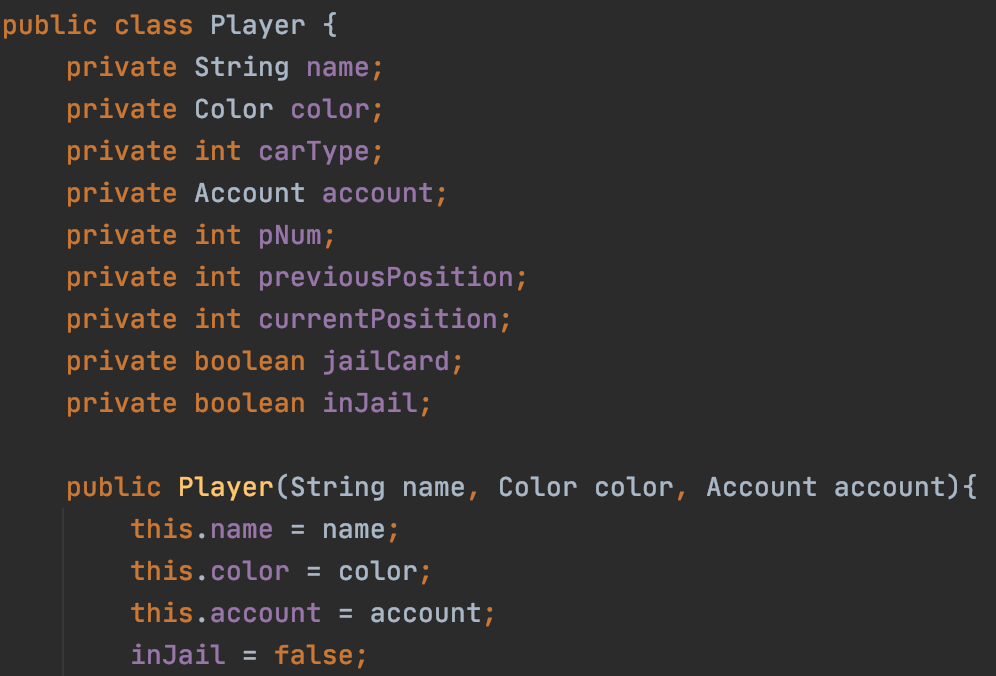
\includegraphics[width=\textwidth]{sources/7_implementering/Player Properties.png}
    \caption{Player variable}
    \label{fig:playVariable}
\end{figure}
En spiller bliver oprettet med et navn, account og farve. Det bruges til at holde styr på dem hver for sig.

Der er en isInJail metode, som holder styr på om spilleren sidder i fængsel. Den brugs i logikken, når spillet skal vide, om en spiller bevæger sig frit på banen, eller først skal ud af fængsel.
\begin{figure}[H]
    \centering
    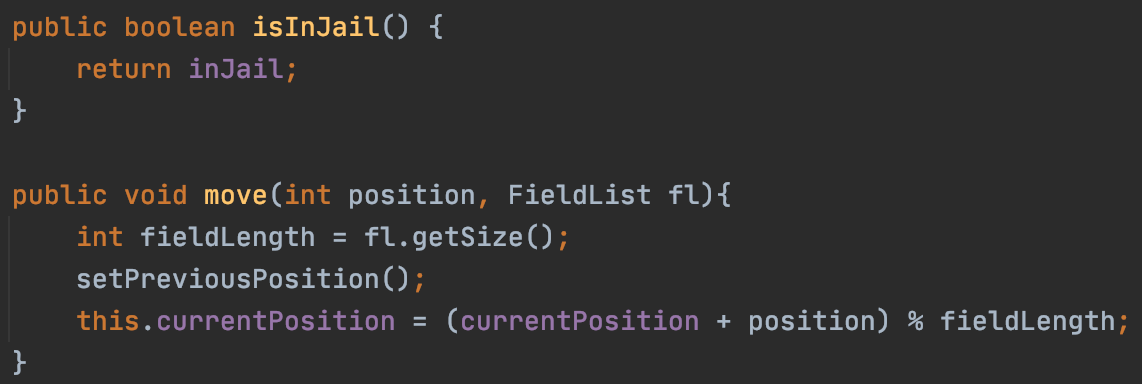
\includegraphics[width=\textwidth]{sources/7_implementering/Player isInJail.png}
    \caption{isInJail Metode}
    \label{fig:isInJail}
\end{figure}

Move-metoden får spilleren til at bevæge sig, ved at kende til brættet og spillerens position. Den bruges, når spilleren skal i fængsel eller har kastet og blot skal flytte sin brik.

setOutOfJailCard og isJailCard holder styr på spillerens kort, for at komme ud af fængsel, og sørger for, at man kan tildele dette kort samt fjerne det fra spilleren, når det er brugt.
\begin{figure}[H]
    \centering
    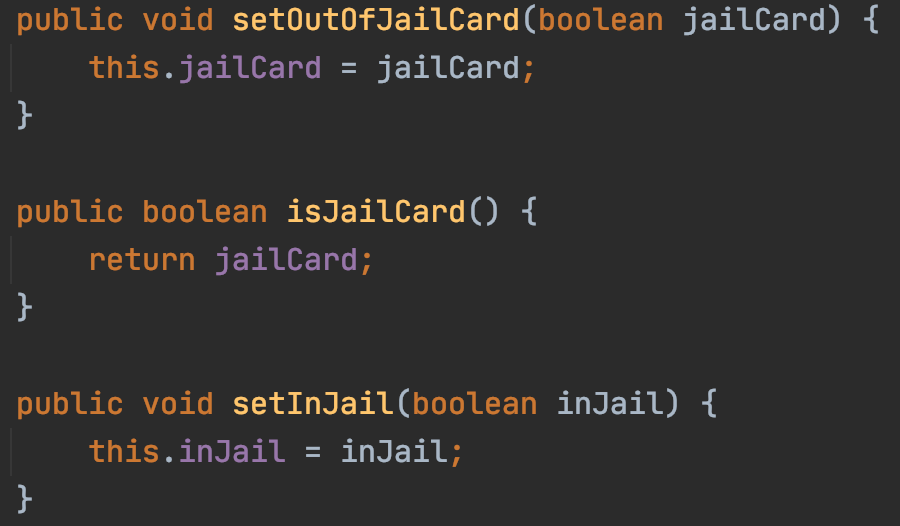
\includegraphics[width=\textwidth]{sources/7_implementering/Player JailRelated.png}
    \caption{Player - Jail Related }
    \label{fig:PlayerJail}
\end{figure}

Herefter er en række getters og setters for information omkring spilleren, som bruges i logikken og gui'en.
\begin{figure}[H]
    \centering
    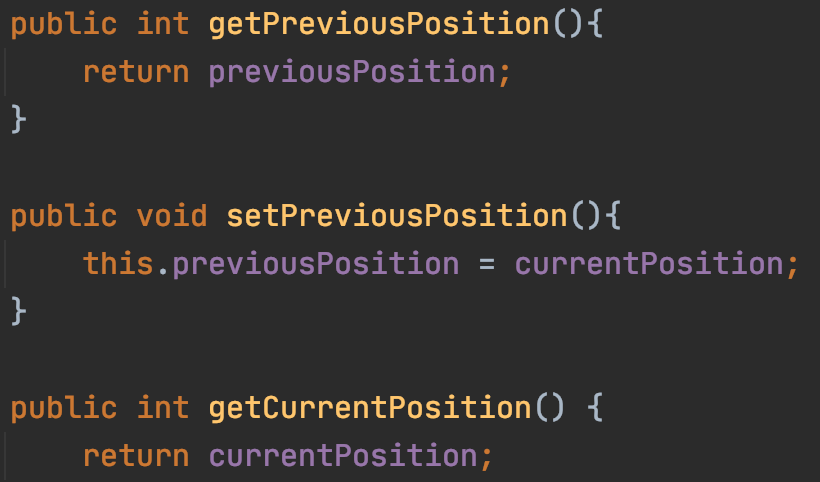
\includegraphics[width=\textwidth]{sources/7_implementering/Player Position.png}
    \caption{}
    \label{fig:}
\end{figure}